% Copyright 2020-2024 Robert Bosch GmbH

% Licensed under the Apache License, Version 2.0 (the "License");
% you may not use this file except in compliance with the License.
% You may obtain a copy of the License at

% http://www.apache.org/licenses/LICENSE-2.0

% Unless required by applicable law or agreed to in writing, software
% distributed under the License is distributed on an "AS IS" BASIS,
% WITHOUT WARRANTIES OR CONDITIONS OF ANY KIND, either express or implied.
% See the License for the specific language governing permissions and
% limitations under the License.

% --------------------------------------------------------------------------------------------------------------

\section{How to execute}

The \pkg\ is implemented in Python3 and therefore requires a Python3 installation.

A basic Python script to use the \pkg\ can look like this:

\begin{pythoncode}
from JsonPreprocessor.CJsonPreprocessor import CJsonPreprocessor
import pprint

json_preprocessor = CJsonPreprocessor()
try:
   values = json_preprocessor.jsonLoad("./file.jsonp")
   pprint.pprint(values)
except Exception as reason:
   print(f"'{reason}'")
\end{pythoncode}

The main method of the \pkg\ is: \pcode{jsonLoad}. Input is the path and the name of a JSON file.
Output is a dictionary containing all values parsed from this JSON file.

In case of any errors while computing the JSON file, the \pkg\ throws an exception. Therefore it is required
to call the method \pcode{jsonLoad} inside a \pcode{try/except} block.

\pcode{pprint} is used in this example to give the output a better readability in console.

\vspace{2ex}

In chapter \hyperref[thejsonpformat]{The JSONP format} the format of JSON files used by the \pkg, is described in detail.
All discussed JSON files can be tested with the example script listed above.

% --------------------------------------------------------------------------------------------------------------

\newpage

\section{User defined naming convention}

By default, key names in JSON files can contain any characters (but cannot be empty). But it might be required to limit the character set.
For this purpose the \pkg\ supports an optional user-defined convention for key names. This is enforced using a \pcode{regex} pattern
passed to the constructor of the \pkg\ class.

Assuming key names may only contain letters, digits and underscores, but must start with a letter, then the \pkg\ has to be initialized
in this way:

\begin{pythoncode}[linebackgroundcolor=\hlcode{3,5}]
from JsonPreprocessor.CJsonPreprocessor import CJsonPreprocessor
import pprint
import regex

json_preprocessor = CJsonPreprocessor(keyPattern=r'^\p{L}[\p{L}\p{Nd}_]*$'))
try:
   values = json_preprocessor.jsonLoad("./file.jsonp")
   pprint.pprint(values)
except Exception as reason:
   print(f"'{reason}'")
\end{pythoncode}

The regular expressions \pcode{\\p\{L\}} and \pcode{\\p\{Nd\}} are provided by the \pcode{regex} module:

\begin{itemize}
   \item \pcode{\\p\{L\}} matches all Unicode characters classified as \textbf{letter}
   \item \pcode{\\p\{Nd\}} matches all Unicode characters classified as \textbf{decimal digit}
\end{itemize}

% --------------------------------------------------------------------------------------------------------------

\newpage

\section{VSCodium support}

In the introduction we mentioned that the JSON syntax extensions introduced by the \pkg, harm the syntax highlighting of editors.

Either we give the JSON files the extension \pcode{.json}, then an editor expects a JSON file in standard syntax,
or we change the extension to \pcode{.jsonp}, but in this case an editor usually does not know how to display a file of such type.

In case you use \href{https://vscodium.com/}{VSCodium}, you can install a
\href{https://github.com/test-fullautomation/vscode-jsonp}{jsonp extension}. 

With this extension the VSCodium editor will be able to display \pcode{.jsonp} files properly.

\vspace{2ex}

\textbf{Some Impressions:}

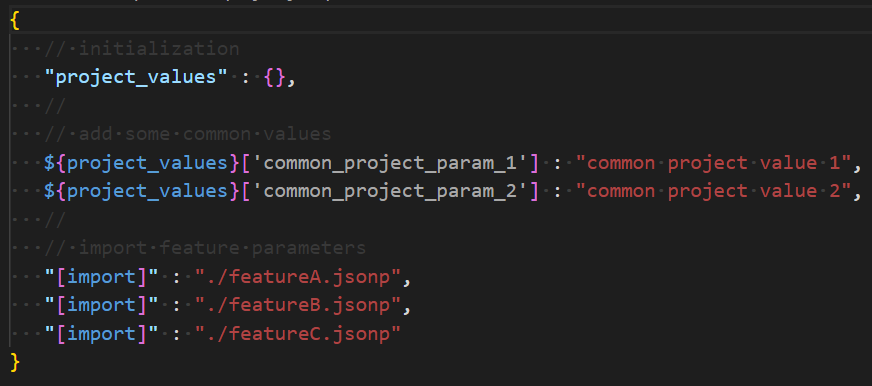
\includegraphics{./pictures/screenshot1.png}

\vspace{2ex}

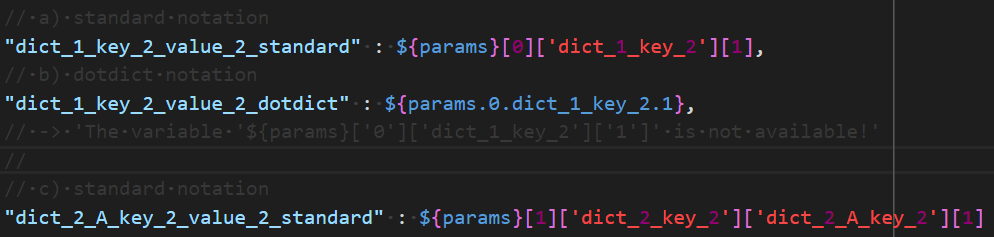
\includegraphics{./pictures/screenshot2.png}

% --------------------------------------------------------------------------------------------------------------
